\documentclass[12pt]{article}
\usepackage[left=1cm, right=1cm, top=2cm,bottom=1.5cm]{geometry} 

\usepackage[parfill]{parskip}
\usepackage[utf8]{inputenc}
\usepackage[T2A]{fontenc}
\usepackage[russian]{babel}
\usepackage{enumitem}
\usepackage[normalem]{ulem}
\usepackage{amsfonts, amsmath, amsthm, amssymb, mathtools,xcolor}
\usepackage{blkarray}

\usepackage{tabularx}
\usepackage{hhline}

\usepackage{accents}
\usepackage{fancyhdr}
\pagestyle{fancy}
\renewcommand{\headrulewidth}{1.5pt}
\renewcommand{\footrulewidth}{1pt}

\usepackage{graphicx}
\usepackage[figurename=Рис.]{caption}
\usepackage{subcaption}
\usepackage{float}

%%Наименование папки откуда забирать изображения
\graphicspath{ {./images/} }

%%Изменение формата для ввода доказательства
\renewcommand{\proofname}{$\square$  \nopunct}
\renewcommand\qedsymbol{$\blacksquare$}

%%Изменение отступа на таблицах
\addto\captionsrussian{%
	\renewcommand{\proofname}{$\square$ \nopunct}%
}
%% Римские цифры
\newcommand{\RN}[1]{%
	\textup{\uppercase\expandafter{\romannumeral#1}}%
}

%% Для удобства записи
\newcommand{\MR}{\mathbb{R}}
\newcommand{\MC}{\mathbb{C}}
\newcommand{\MQ}{\mathbb{Q}}
\newcommand{\MN}{\mathbb{N}}
\newcommand{\MZ}{\mathbb{Z}}
\newcommand{\MTB}{\mathbb{T}}
\newcommand{\MTI}{\mathbb{I}}
\newcommand{\MI}{\mathrm{I}}
\newcommand{\MCI}{\mathcal{I}}
\newcommand{\MJ}{\mathrm{J}}
\newcommand{\MH}{\mathrm{H}}
\newcommand{\MT}{\mathrm{T}}
\newcommand{\MU}{\mathcal{U}}
\newcommand{\MV}{\mathcal{V}}
\newcommand{\MB}{\mathcal{B}}
\newcommand{\MF}{\mathcal{F}}
\newcommand{\MW}{\mathcal{W}}
\newcommand{\ML}{\mathcal{L}}
\newcommand{\MP}{\mathcal{P}}
\newcommand{\VN}{\varnothing}
\newcommand{\VE}{\varepsilon}
\newcommand{\dx}{\, dx}
\newcommand{\dy}{\, dy}
\newcommand{\dz}{\, dz}
\newcommand{\dd}{\, d}


\theoremstyle{definition}
\newtheorem{defn}{Опр:}
\newtheorem{rem}{Rm:}
\newtheorem{prop}{Утв.}
\newtheorem{exrc}{Упр.}
\newtheorem{problem}{Задача}
\newtheorem{lemma}{Лемма}
\newtheorem{theorem}{Теорема}
\newtheorem{corollary}{Следствие}

\newenvironment{cusdefn}[1]
{\renewcommand\thedefn{#1}\defn}
{\enddefn}

\DeclareRobustCommand{\divby}{%
	\mathrel{\text{\vbox{\baselineskip.65ex\lineskiplimit0pt\hbox{.}\hbox{.}\hbox{.}}}}%
}
\DeclareRobustCommand{\ndivby}{\mkern-1mu\not\mathrel{\mkern4.5mu\divby}\mkern1mu}


%Короткий минус
\DeclareMathSymbol{\SMN}{\mathbin}{AMSa}{"39}
%Длинная шапка
\newcommand{\overbar}[1]{\mkern 1.5mu\overline{\mkern-1.5mu#1\mkern-1.5mu}\mkern 1.5mu}
%Функция знака
\DeclareMathOperator{\sgn}{sgn}

%Функция ранга
\DeclareMathOperator{\rk}{\text{rk}}
\DeclareMathOperator{\diam}{\text{diam}}


%Обозначение константы
\DeclareMathOperator{\const}{\text{const}}

\DeclareMathOperator{\codim}{\text{codim}}

\DeclareMathOperator*{\dsum}{\displaystyle\sum}
\newcommand{\ddsum}[2]{\displaystyle\sum\limits_{#1}^{#2}}
\newcommand{\ddssum}[2]{\displaystyle\smashoperator{\sum\limits_{#1}^{#2}}}
\newcommand{\ddlsum}[2]{\displaystyle\smashoperator[l]{\sum\limits_{#1}^{#2}}}
\newcommand{\ddrsum}[2]{\displaystyle\smashoperator[r]{\sum\limits_{#1}^{#2}}}

%Интеграл в большом формате
\DeclareMathOperator{\dint}{\displaystyle\int}
\newcommand{\ddint}[2]{\displaystyle\int\limits_{#1}^{#2}}
\newcommand{\ssum}[1]{\displaystyle \sum\limits_{n=1}^{\infty}{#1}_n}

\newcommand{\smallerrel}[1]{\mathrel{\mathpalette\smallerrelaux{#1}}}
\newcommand{\smallerrelaux}[2]{\raisebox{.1ex}{\scalebox{.75}{$#1#2$}}}

\newcommand{\smallin}{\smallerrel{\in}}
\newcommand{\smallnotin}{\smallerrel{\notin}}

\newcommand*{\medcap}{\mathbin{\scalebox{1.25}{\ensuremath{\cap}}}}%
\newcommand*{\medcup}{\mathbin{\scalebox{1.25}{\ensuremath{\cup}}}}%

\makeatletter
\newcommand{\vast}{\bBigg@{3.5}}
\newcommand{\Vast}{\bBigg@{5}}
\makeatother

%Промежуточное значение для sup\inf, поскольку они имеют разную высоту
\newcommand{\newsup}{\mathop{\smash{\mathrm{sup}}}}
\newcommand{\newinf}{\mathop{\mathrm{inf}\vphantom{\mathrm{sup}}}}

%Скалярное произведение
\newcommand{\inner}[2]{\left\langle #1, #2 \right\rangle }
\newcommand{\linsp}[1]{\left\langle #1 \right\rangle }
\newcommand{\linmer}[2]{\left\langle #1 \vert #2\right\rangle }

%Подпись символов снизу
\newcommand{\ubar}[1]{\underaccent{\bar}{#1}}

%%Шапка для букв сверху
\newcommand{\wte}[1]{\widetilde{#1}}
\newcommand{\wht}[1]{\widehat{#1}}
\newcommand{\ovl}[1]{\overline{#1}}


%%Трансформация Фурье
\newcommand{\fourt}[1]{\mathcal{F}\left(#1\right)}
\newcommand{\ifourt}[1]{\mathcal{F}^{-1}\left(#1\right)}

%%Символ вектора
\newcommand{\vecm}[1]{\overrightarrow{#1\,}}

%%Пространстов матриц
\newcommand{\matsq}[1]{\operatorname{Mat}_{#1}}
\newcommand{\mat}[2]{\operatorname{Mat}_{#1, #2}}

%Оператор для действ и мнимых чисел
\DeclareMathOperator{\IM}{\operatorname{Im}}
\DeclareMathOperator{\RE}{\operatorname{Re}}
\DeclareMathOperator{\li}{\operatorname{li}}
\DeclareMathOperator{\GL}{\operatorname{GL}}
\DeclareMathOperator{\SL}{\operatorname{SL}}
\DeclareMathOperator{\Char}{\operatorname{char}}
\DeclareMathOperator\Arg{Arg}
\DeclareMathOperator\ord{ord}

%Оператор для образа
\DeclareMathOperator{\Ima}{Im}

%Делимость чисел
\newcommand{\modn}[3]{#1 \equiv #2 \; (\bmod \; #3)}
\newcommand{\nmodn}[3]{#1 \not\equiv #2 \; (\bmod \; #3)}

%%Взятие в скобки, модули и норму
\newcommand{\parfit}[1]{\left( #1 \right)}
\newcommand{\modfit}[1]{\left| #1 \right|}
\newcommand{\sqparfit}[1]{\left\{ #1 \right\}}
\newcommand{\normfit}[1]{\left\| #1 \right\|}

%%Функция для обозначения равномерной сходимости по множеству
\newcommand{\uconv}[1]{\overset{#1}{\rightrightarrows}}
\newcommand{\uconvm}[2]{\overset{#1}{\underset{#2}{\rightrightarrows}}}


%%Функция для обозначения нижнего и верхнего интегралов
\def\upint{\mathchoice%
	{\mkern13mu\overline{\vphantom{\intop}\mkern7mu}\mkern-20mu}%
	{\mkern7mu\overline{\vphantom{\intop}\mkern7mu}\mkern-14mu}%
	{\mkern7mu\overline{\vphantom{\intop}\mkern7mu}\mkern-14mu}%
	{\mkern7mu\overline{\vphantom{\intop}\mkern7mu}\mkern-14mu}%
	\int}
\def\lowint{\mkern3mu\underline{\vphantom{\intop}\mkern7mu}\mkern-10mu\int}

%%След матрицы
\DeclareMathOperator*{\tr}{tr}

\makeatletter
\renewcommand*\env@matrix[1][*\c@MaxMatrixCols c]{%
	\hskip -\arraycolsep
	\let\@ifnextchar\new@ifnextchar
	\array{#1}}
\makeatother


%% Переопределение функции хи, чтобы выглядела более приятно
\makeatletter
\@ifdefinable\@latex@chi{\let\@latex@chi\chi}
\renewcommand*\chi{{\@latex@chi\smash[t]{\mathstrut}}} % want only bottom half of \mathstrut
\makeatletter

\setcounter{MaxMatrixCols}{20}
\begin{document}
\lhead{Алгебра-\RN{1}}
\chead{Тимашев Д.А.}
\rhead{Лекция - 24}
\section*{Начала теории групп}
\begin{defn}
	\uwave{Группа} - это множество $G$, на котором задана \uwave{бинарная операция} $\cdot \colon G \times G \to G$, обычно называемая \uwave{умножением}, которая должна удовлетворять свойствам, называемыми \uline{аксиомами группы}:
	\begin{enumerate}[label=\arabic*)]
		\item \textbf{Ассоциативность}: 
		$$
			\forall a,b,c \in G,\, (a \cdot b)\cdot c = a\cdot (b \cdot c)
		$$
		\item \textbf{Существование нейтрального элемента}: 
		$$	
			\exists \, e \in G \colon \forall g \in G, \, g \cdot e = e \cdot g = g
		$$
		где $e$ - \uwave{нейтральный элемент} или ещё его называют \uwave{единицей} в группе $G$;
		\item \textbf{Существование обратного элемента}:
		$$
			\forall a \in G, \, \exists \, b \in G \colon a \cdot b = b \cdot a = e	
		$$
		где $b$ - \uwave{обратный элемент} к элементу $a$.
		
		\textbf{\uline{Обозначение}}: $b = a^{-1}$;
	\end{enumerate}
\end{defn}

\begin{defn}
	Подмножество $H \subseteq G$ называется \uwave{подгруппой}, если $e \in H$ и $\forall a,b \in H, \, ab^{-1} \in H$.
\end{defn}
\begin{prop}
	$$
		\forall a,b \in H, \, ab^{-1} \in H \Leftrightarrow
		\begin{cases}
			\forall a,b \in H, & ab \in H \\
			\forall a \in H, & a^{-1} \in H
		\end{cases}
	$$
\end{prop}
\begin{proof}\hfill\\
	$(\Rightarrow)$ $\forall a,b\in H ab^{-1} \in H \Rightarrow \forall b \in H, \, eb^{-1} = b^{-1} \in H$, $\forall a,b^{-1} \in H, \, a(b^{-1})^{-1} = ab \in H$.
	
	$(\Leftrightarrow)$ $\forall a,b \in H, \, ab \in H, \, a^{-1} \in H \Rightarrow b^{-1} \in H,\, \Rightarrow ab^{-1} \in H$.
\end{proof}

\begin{rem}
	Подгруппа это подмножество, которое само является группой относительно той же операции.
\end{rem}

\begin{defn}
	Подгруппы $H = \{e\} \subseteq G, \, H = G \subseteq G$ называются \uwave{несобственными}. Группы отличные от несобственных называются \uwave{собственными}.
\end{defn}

\begin{rem}
	В любой группе $G$ всегда есть несобственные подгруппы.
\end{rem}

\textbf{Пример подгруппы}: $G = (\MZ, +)$, тогда $H = \{-1,1\}$ - не подгруппа, поскольку не содержит $0$. При этом это является группой относительно умножения.

Как проверить, что $H \subseteq G$ является подгруппой? Необходимо проверить свойства группы, при этом ассоциативность проверять не нужно, потому что $H$ это подмножество $G$, в котором для любых элементов выполнено свойство ассоциативности.

\textbf{Пример подгрупп}: Пусть $G = (\MZ, +)$, тогда $H = n\MZ$, где $n$ - фиксировано, $n \in \MZ_{\geq 0}$.
\begin{enumerate}[label=\arabic*)]
	\item $n = 0 \Rightarrow n\MZ = 0 = \{e\}$;
	\item $n = 1 \Rightarrow n\MZ = \MZ$;
	\item $n = 2 \Rightarrow n\MZ = 2\MZ$ - чётные;
\end{enumerate}
Таким образом, мы можем прийти к следующему предложению.

\begin{prop}
	Любая подгруппа в $(\MZ,+)$ имеет вид $n\MZ, \, n \in \MZ_{\geq 0}$.
\end{prop}
\begin{rem}
	$n \in \MZ_{\geq 0}$, поскольку подгруппа, например, $-3\MZ$ совпадает с подгруппой $3\MZ$.
\end{rem}
\begin{proof}\hfill\\
	$(\Leftarrow)$ Ясно, что $n\MZ$ - подгруппа.
	
	$(\Rightarrow)$ Пусть $H \subseteq G$ - некоторая подгруппа. Если $H = \{0\}$, то $n = 0$. Если $H \neq \{0\}$, то: 
	$$
		\exists \, a\in H, a \neq 0 \Rightarrow \pm a \in H \Rightarrow \exists \, a \in H, a > 0
	$$
	Пусть $n \in \MN$ - наименьшее, лежащее в $H \Rightarrow n\MZ \subseteq H$. Разделим $a \in H$  с остатком на $n$:
	$$
		a = nq + r, \, 0 \leq r < n, \, r = a - nq \in H \Rightarrow r = 0
	$$
	так как $n$ - минимальный положительный $\Rightarrow H = n\MZ$, поскольку каждый элемент подгруппы $H$ представим в виде $nq$ для некоторого $q \in \MZ$.
\end{proof}

\begin{defn}
	Пусть $(G, \circ)$ и $(H, *)$ - группы, тогда \uwave{гомоморфизм} $\varphi \colon G \to H$ это отображение вида:
	$$
		\forall a,b \in G, \, \varphi(a\circ b) = \varphi(a)*\varphi(b)
	$$
\end{defn}
\begin{prop}
	Для гомоморфизма будет верно:
	\begin{enumerate}[label=\arabic*)]
		\item $e_G \in G, \, e_H \in H \Rightarrow \varphi(e_G) = e_H$;
		\item $\varphi(a^{-1}) = \varphi(a)^{-1}$;
	\end{enumerate}
\end{prop}
\begin{proof}\hfill
	\begin{enumerate}[label=\arabic*)]
		\item $\forall a \in G, \, \varphi(a) = \varphi(a\circ e_G) = \varphi(a)*\varphi(e_G) \Rightarrow \varphi(a)^{-1}*\varphi(a) = \varphi(a)^{-1}*\varphi(a)*\varphi(e_G) \Rightarrow e_H = \varphi(e_G)$;
		\item $\forall a \in G, \, \varphi(a \circ a^{-1}) = \varphi(e_G) \Rightarrow \varphi(a)^{-1}*e_H = \varphi(a)^{-1}= \varphi(a)^{-1}*\varphi(a)*\varphi(a^{-1}) = e_H*\varphi(a^{-1}) = \varphi(a^{-1})$;
	\end{enumerate}
\end{proof}

\subsection*{Порядок элемента группы}

\begin{defn}
	\uwave{Возведение элемента $g \in G$ в степень} $n \in \MZ$: $g^n = 
		\begin{cases}
			\underbrace{g{\cdot}\dotsc{\cdot}g}_{n}, & n > 0\\
			\underbrace{g^{-1}{\cdot}\dotsc{\cdot}g^{-1}}_{|n|}, & n < 0\\
			e, & n = 0
		\end{cases}$.
\end{defn}

\begin{prop}\textbf{\uline{Свойства возведения в степень}}:
	\begin{enumerate}[label=\arabic*)]
		\item $g^n{\cdot}g^m = g^{n + m}$;
		\item $(g^n)^m = g^{nm}$;
	\end{enumerate}
\end{prop}
\begin{proof}\hfill
	\begin{enumerate}[label=\arabic*)]
		\item Рассмотрим возможные случаи:
		\begin{enumerate}[label=(\arabic*)]
			\item $n, m > 0 \Rightarrow g^ng^m = \underbrace{g{\cdot}\dotsc{\cdot}g}_{n}{\cdot}\underbrace{g{\cdot}\dotsc{\cdot}g}_{m} = \underbrace{g{\cdot}\dotsc{\cdot}g}_{n + m} = g^{n + m}$;
			\item $n, m < 0 \Rightarrow g^ng^m =  \underbrace{g^{-1}{\cdot}\dotsc{\cdot}g^{-1}}_{|n|}{\cdot}\underbrace{g^{-1}{\cdot}\dotsc{\cdot}g^{-1}}_{|m|} = \underbrace{g^{-1}{\cdot}\dotsc{\cdot}g^{-1}}_{|n| + |m|} = \underbrace{g^{-1}{\cdot}\dotsc{\cdot}g^{-1}}_{|n + m|} = g^{nm}$;
			\item $n > |m| > 0, m < 0\Rightarrow g^ng^m = \underbrace{g{\cdot}\dotsc{\cdot}g}_{n}{\cdot}\underbrace{g^{-1}{\cdot}\dotsc{\cdot}g^{-1}}_{|m|} = \underbrace{g{\cdot}\dotsc{\cdot}g}_{n - |m|}{\cdot}\underbrace{e{\cdot}\dotsc{\cdot}e}_{|m|} = \underbrace{g{\cdot}\dotsc{\cdot}g}_{n + m} = g^{n + m}$;
			\item $|m| > n > 0, m < 0\Rightarrow g^ng^m = \underbrace{g{\cdot}\dotsc{\cdot}g}_{n}{\cdot}\underbrace{g^{-1}{\cdot}\dotsc{\cdot}g^{-1}}_{|m|} = \underbrace{e{\cdot}\dotsc{\cdot}e}_{n}{\cdot}\underbrace{g^{-1}{\cdot}\dotsc{\cdot}g^{-1}}_{|m| - n} = \underbrace{g^{-1}{\cdot}\dotsc{\cdot}g^{-1}}_{|m + n|} = g^{n + m}$;
			\item $n,m = 0 \Rightarrow g^ng^m = ee = e = g^{n + m}$;
		\end{enumerate}
		
		\item Отметим,что $(g^n)^-1 = g^{-n}$, поскольку: 
		$$
			g^n{\cdot}g^{-n} = g^{-n}{\cdot}g^n = g^{n - n} = g^{0} = e
		$$ 
		Рассмотрим возможные случаи:
		\begin{enumerate}[label=(\arabic*)]
			\item $m > 0 \Rightarrow (g^n)^m =  \underbrace{g^n{\cdot}\dotsc{\cdot}g^n}_{m} = g^{n + n + \dotsc  + n} = g^{nm}$;
			\item $m < 0 \Rightarrow (g^n)^m = \underbrace{(g^n)^{-1}{\cdot}\dotsc{\cdot}(g^n)^{-1}}_{|m|} =\underbrace{g^{-n}{\cdot}\dotsc{\cdot}g^{-n}}_{|m|}=  g^{-n - n - \dotsc -n} = g^{-|m|n} = g^{mn}$;
			\item $m = 0 \Rightarrow (g^n)^0 = e = g^{n{\cdot}0} = g^{nm}$;
		\end{enumerate}

	\end{enumerate}
\end{proof}

Если мы возьмем элемент $g\in G$ и начнём возводить в степени, то возможны две ситуации:
\begin{enumerate}[label=\arabic*)]
	\item Все $g^n$ различны при разных $n \in \MZ$;
	\item Существуют повторения: $g^k = g^l$ при некоторых $k > l, \, k,l \in \MZ$. В этом случае, если домножить левую и правую части на $g^{-l}$, то получим:
	$$
		m = k - l \in \MN, \, g^{m} = g^{k - l} = e
	$$
\end{enumerate}

\begin{defn}
	\uwave{Порядок элемента} $g \in G$ это наименьшое $m \in \MN$ для которого $g^m = e$ или $\infty$, если такого $m$ не существует.
\end{defn}
\textbf{\uline{Обозначение}}: $o(g)$ или $\ord(g)$.

\textbf{Примеры порядков элементов}:
\begin{enumerate}[label=\arabic*)]
	\item \textbf{Цикл длины $l$}: $\sigma = (i_1, i_2,\dotsc,i_l) \in S_n$. Элементы орбиты: $i_1 \to i_2 \to \dotsc \to i_l \to i_1$, все остальные элементы: $i \to i$. Каков порядок такой подстановки? Под действием $\sigma$ каждый элемент сдвигается в следующий по циклу $\Rightarrow$ можем применить подстановку несколько раз, тогда:
	$$
		\sigma^m = \VE \Leftrightarrow m \divby l \Rightarrow \ord(\sigma) = l
	$$
	\item \textbf{Произвольная подстановка $\sigma \in S_n$}: По теореме о разложении на независимые циклы, будет верно:
	$$
		\sigma = \sigma_1{\cdot}\dotsc{\cdot}\sigma_s \Rightarrow \sigma^m = \sigma_1^m{\cdot}\dotsc{\cdot}\sigma_s^m, \, \sigma^m = \VE \Leftrightarrow \sigma_1^m = \dotsc  =\sigma_s^m = \VE \Leftrightarrow m \divby l_1, l_2,\dotsc l_s
	$$
	где $l_1,\dotsc,l_s$ - их длины $\Rightarrow$ у нас несколько непересекающихся орбит разных длин и чтобы найти порядок $\sigma$ мы должны найти наименьшее $m \in \MN$, которое делится на длины всех этих орбит:
	$$
		\ord(\sigma) = [l_1,\dotsc, l_s] = \text{НОК}(l_1,\dotsc, l_s)
	$$
	\item $G = (\MZ, +)$, тогда: $\forall a \in \MZ, \, a \neq 0 \Rightarrow \ord(a) = \infty,\, \ord(0) = 1$; 
\end{enumerate}

\begin{prop}(\textbf{Свойства порядка}) Пусть $g \in G$ - элемент группы, $\ord(g) = m \in \MN$ или $\infty$, тогда:
	\begin{enumerate}[label=\arabic*)]
		\item $g^n = e \Leftrightarrow n \divby m$ или $n = 0$;
		\item $g^k = g^l \Leftrightarrow \modn{k}{l}{m}$ или $k = l$;
	\end{enumerate}
\end{prop}
\begin{proof}\hfill
	\begin{enumerate}[label=\arabic*)]
		\item При $\ord(g) = \infty$ это очевидно, поскольку $g^0 = e$, а остальные $g^n, \, n \neq 0$ это другие элементы группы. При $\ord(g)= m \in \MN$, поделим $n$ с остатком: $n = mq + r, \, 0 \leq r < m$, тогда:
		$$
			 g^n = g^{mq + r} = (g^m)^q{\cdot}g^r =e^q{\cdot}g^r = e{\cdot}g^r = g^r
		$$
		$$
			g^n = e \Leftrightarrow g^r = e \Leftrightarrow r = 0 \Leftrightarrow n \divby m
		$$
		где второе верно, поскольку $m$ - наименьшее натуральное для которого $g^m = e$, а $0 \leq r < m$;
		\item Воспользуемся результатами предыдущего пункта:
		$$
			g^k = g^l \Leftrightarrow g^{k - l} = e \Leftrightarrow k - l \divby m \vee k - l =0 \Leftrightarrow \modn{k}{l}{m} \vee k = l
		$$
		таким образом, что для конечного, что для бесконечного порядка мы доказали равносильность;
	\end{enumerate}
\end{proof}

\subsection*{Изоморфизм групп}
Вспомним немного про изоморфизм. Пусть $(G,\circ), \, (H, *)$ - группы. $\varphi \colon G \to H$ - гомоморфизм:
$$
	\forall a,b \in G, \, \varphi(a \circ b) = \varphi(a)*\varphi(b) 
$$
\begin{defn}
	\uwave{Изоморфизм} это биективный гомоморфизм.
\end{defn}

\begin{prop}
	Для изоморфизма $\varphi \colon G \to H$ верно:
	$$
		\exists\, \varphi^{-1} \colon H \to G, \, \forall c,d \in H, \, \varphi^{-1}(cd) = \varphi^{-1}(c)\varphi^{-1}(d)
	$$
\end{prop}
\begin{proof}
	Поскольку $\varphi$ - биекция, то $\exists\, \varphi^{-1} \colon H \to G$. Тогда:
	$$
		\forall c,d \in H, \, \varphi(\varphi^{-1}(c*d)) = c*d = \varphi(\varphi^{-1}(c))\circ\varphi(\varphi^{-1}(d)) = \varphi(\varphi^{-1}(c)\circ\varphi^{-1}(d)) \Rightarrow 
	$$
	$$
		\Rightarrow \varphi^{-1}(c*d) = \varphi^{-1}(c)\circ\varphi^{-1}(d)
	$$
	так как $\varphi$ - биекция.
\end{proof}
\begin{rem}
	Таким образом, изоморфизм это обратимый гомоморфизм, и обратный к нему также будет гомоморфизмом.
\end{rem}

\begin{defn}
	Группы $G$ и $H$ \uwave{изоморфны}, если существует изоморфизм: $\varphi \colon G \to H$.
\end{defn}
\textbf{\uline{Обозначение}}: $G \simeq H$.
\newpage
\textbf{Пример изоморфизма}: $G = (\MR, +), \, H = (\MR^\times,\cdot), \, \varphi \colon G \to H,\, \forall a\in \MR,\, \varphi(a) = e^a$, тогда:
$$
	\forall a,b \in \MR, \, \varphi(a + b) = e^{a + b} = e^ae^b = \varphi(a)\varphi(b)
$$
Следовательно, $\varphi$ - гомоморфизм. $\forall c \in \MR^\times, \, \varphi^{-1}(c) = \ln(c) \Rightarrow \varphi$ - изоморфизм и $G \simeq H$.

С точки зрения теории групп это одна и та же группа, и все утверждения, доказанные для одной из них, также будут верны и для другой. 

\begin{defn}
	\uwave{Эндоморфизм} это гомоморфизм в себя: $\varphi \colon G \to G$.
\end{defn}
\begin{defn}
	\uwave{Автоморфизм} это изоморфизм в себя: $\varphi \colon G \xrightarrow{\sim} G$.
\end{defn}
Очевидно, что каждая группа одинакова сама с собой, но важно понять, сколькими способами можно отождествить группу с собой. Есть группы у которых почти нет автоморфизмов (когда отождествить группу с собой можно единственным способом), а есть группы для которых это можно сделать несколькими способами (аналог замены координат в группе).

\subsection*{Ядро и образ}
\begin{defn}
	Если $\varphi \colon G \to H$ это гомоморфизм, то:
	\begin{enumerate}[label=\arabic*)]
		\item \uwave{Ядром} $\varphi$ называется множество: 
		$$
			\ker\varphi = \{a \in G \mid \varphi(a) = e_H\}
		$$
		\item \uwave{Образом} $\varphi$ называется множество: 
		$$
			\Ima\varphi = \{b \in H \mid \exists \, a \in G \colon \varphi(a) = b\}
		$$
	\end{enumerate}
\end{defn}
\begin{figure}[H]
	\centering
	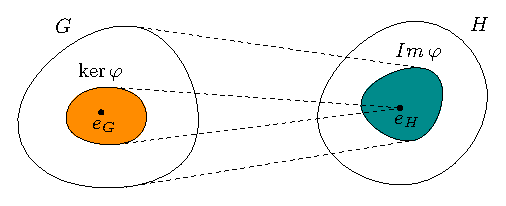
\includegraphics[width=0.55\textwidth]{AL1L24_1.eps}
	\caption{Образ и ядро оператора $\varphi$.}
	\label{24_1}
\end{figure}
\begin{exrc}
	Пусть $\varphi \colon G \to H$ - гомоморфизм, тогда:
	\begin{enumerate}[label=\arabic*)]
		\item $\varphi$ - изоморфизм $\Leftrightarrow \Ima\varphi = H, \, \ker\varphi = \{e_G\}$;
		\item $\ker\varphi \subseteq G, \, \Ima \varphi \subseteq H$ - подгруппы;
	\end{enumerate}
\end{exrc}
\begin{proof}\hfill
	\begin{enumerate}[label=\arabic*)]
		\item $(\Rightarrow)$ $\varphi$ - изоморфизм, тогда $\varphi$ - биекция: 
		$$
			\forall b \in H, \, \exists \, a\in G \colon \varphi(a) = b \Rightarrow H \subseteq \Ima\varphi \Rightarrow \Ima\varphi = H
		$$
		$$
			\forall a \in G,\, \varphi(a\circ e_G) =  \varphi(e_G\circ a) =\varphi(a) = \varphi(a)*\varphi(e_G) = \varphi(e_G)*\varphi(a) \Rightarrow
		$$
		$$
			\Rightarrow \varphi(e_G) = e_H \Rightarrow \ker\varphi = \{e_G\}
		$$
		\newpage
		$(\Leftarrow)$ $\Ima\varphi = H \Rightarrow \varphi$ - сюръекция. Поскольку $\ker\varphi = \{e_G\} \Rightarrow \varphi(e_G) = e_H$, тогда:
		$$
			\forall a,b \in G, \varphi(a) = \varphi(b) \Rightarrow \varphi(a\circ a^{-1}) = \varphi(b\circ a^{-1}) \Rightarrow e_H = \varphi(e_G) = \varphi(b\circ a^{-1}) \Rightarrow
		$$
		$$
			\Rightarrow b\circ a^{-1} \in \ker\varphi \Rightarrow b\circ a^{-1} = e_G \Rightarrow b \circ a^{-1}\circ a = e_G \circ a \Rightarrow b = a
		$$
		Следовательно, $\varphi$ - биекция;
		\item Проверим, что $\ker\varphi \subseteq G$ это подгруппа $G$:
		$$
			\forall a,b \in \ker\varphi, \, \varphi(a\circ b) = \varphi(a)*\varphi(b) = e_H{\cdot}e_H = e_H \Rightarrow a\circ b \in \ker\varphi
		$$
		$$
			\forall a \in \ker\varphi, \, \varphi(a) = e_H \Rightarrow \varphi(a)\varphi(a^{-1}) = e_H\varphi(a^{-1}) \Rightarrow \varphi(e_G) = e_H = \varphi(a^{-1}) \Rightarrow a^{-1} \in \ker\varphi
		$$
		Проверим, что $\Ima\varphi \subseteq H$ это подгруппа $H$:
		$$
			\forall a,b \in \Ima\varphi, \, \exists \, c,d \in G \colon \varphi(c) = a, \, \varphi(d) = b \Rightarrow \varphi(c\circ d) = a * b
		$$
		$$
			a* b \in H,\, c \circ d \in G, \, \varphi(c\circ d) = a * b \Rightarrow a * b \in \Ima\varphi
		$$
		$$
			\forall a \in \Ima\varphi, \, \exists \, c \in G \colon \varphi(c) = a, \, a \in H, \, c\in G \Rightarrow \exists \, a^{-1} \in H, \, \exists \, c^{-1} \in G \Rightarrow
		$$
		$$	
			a*a^{-1} = a^{-1}*a = \varphi(c)*a^{-1} = a^{-1}*\varphi(c) = e_H \Rightarrow
		$$
		$$
			\Rightarrow \varphi(c^{-1})*\varphi(c)*a^{-1} = \varphi(c^{-1})*e_H \Rightarrow \varphi(e_G)*a^{-1} = a^{-1} = \varphi(c^{-1}) \Rightarrow a^{-1} \in \Ima\varphi
		$$
	\end{enumerate}
\end{proof}

\subsection*{Примеры групп}
\begin{enumerate}[label=\arabic*)]
	\item \textbf{Числовые аддитивные группы}: $(\MR, +), \, (\MQ, +), \, (\MZ, +), \, (\MC, +)$
	это всё примеры бесконечных групп, $(\MZ_n, +)$ - пример конечной аддитивной группы. Все эти группы коммутативны;
	\item \textbf{Числовые мультипликативные группы}: $(\MZ^\times, {\cdot}) = \{-1,1\}$, $(F^\times, \cdot)$, где  $F^\times = F\setminus \{0\}$ и $F$ - любое поле, $(\MZ_n^\times,\cdot)$, где $\MZ_n^\times = \{\ovl{k}\mid (k,n) = 1\}$. Все эти группы коммутативны;
	\item \textbf{Группа подстановок}: $S_n$ - симметрическая группа, $A_n \subseteq S_n$ - группа четных подстановок или знакопеременная группа (alternating group);
	\item \textbf{Группа Клейна}: 
	$$
		V_4 = \{id, (12)(34), (13)(24), (14)(23)\} \subseteq S_4
	$$
	Для подстановок длины $4$ все пары независимых циклов оказываются подгруппой. Каждый элемент обратен сам к себе, а произведение двух подстановок равняется третьей. Это уникальное свойство $S_4$. Например, в $S_5$ пары независимых циклов уже не образуют подгруппу;
	\item \textbf{Группа матриц} (по умножению):
	\begin{enumerate}[label=(\arabic*)]
		\item $GL_n(F) =\{A \in \mat{n}{n} \mid \det(A) \neq 0\}$ \uwave{полная линейная группа} над полем $F$;
		\item $SL_n(F) =\{A \in \mat{n}{n} \mid \det(A) = 1\} \subseteq GL_n(F)$ \uwave{специальная линейная группа} над полем $F$;
		\item $D_n(F) = \left\{A \in \mat{n}{n} \bBigg@{3}| A =
		\begin{pmatrix}
			* & 0  & 0 \\
			0 & \ddots & 0\\
			0 & 0 & *
		\end{pmatrix} \right\}$ \uwave{диагональные матрицы}.
	
		Заметим, что на диагонали должны стоять ненулевые элементы для обратимости;
		\item $B_n(F) = \left\{A \in \mat{n}{n} \bBigg@{3}| A =
		\begin{pmatrix}
			* & *  & * \\
			0 & \ddots & *\\
			0 & 0 & *
		\end{pmatrix} \right\}$ \uwave{верхнетреугольные матрицы}.
	
	 	Заметим,что на диагонали должны стоять ненулевые элементы для обратимости, над диагональю - произвольные элементы;
		\item $U_n(F) = \left\{A \in \mat{n}{n} \bBigg@{3}| A =
		\begin{pmatrix}
			1 & *  & * \\
			0 & \ddots & *\\
			0 & 0 & 1
		\end{pmatrix} \right\}$ \uwave{унитреугольные матрицы};
	\end{enumerate}
	\item \textbf{Группа кватернионов}: $Q_8 = \{\pm1, \pm i, \pm j, \pm k\}, \, i^2 = j^2 = k^2 = -1$, определим умножение по цепочке:
	$$
		ij = k, \, jk = i, \, ki = j,\, ji = -k, \, ik = -j, \, kj = -i
	$$
	\begin{figure}[H]
		\centering
		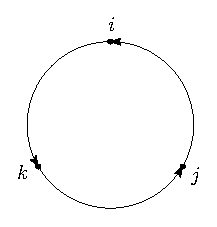
\includegraphics[width=0.2\textwidth]{AL1L24_2.eps}
		\caption{Умножение в группе кватернионов.}
		\label{24_2}
	\end{figure}
	Если идти против часовой стрелки, то перемножение соседних элементов даст следующий элемент со знаком $+$, если перемножать по часовой стрелке, то со знаком минус;
\end{enumerate}


\subsection*{Циклические группы}
Пусть $g \in G$, рассмотрим множество, состоящее из всех степеней $g$: $H = \{g^n \mid n \in \MZ\}$. Это множество замкнуто относительно умножения и взятия обратного элемента, то есть это подгруппа $G$.

\begin{defn}
	\uwave{Множеством всех степеней элемента} $g \in G$ называется множество: $H = \{g^n \mid n \in \MZ\} \subseteq G$.
\end{defn}
\textbf{\uline{Обозначение}}: $H = \linsp{g}$. Если $\ord(g) = m$, то $H = \linsp{g}_m$. Если $\ord(g) = \infty$, то $H = \linsp{g}_{\infty}$.
\begin{rem}
	Множество $H = \linsp{g}, \, g \in G$ также ещё называется \uwave{циклической подгруппой} $G$ и это самая маленькая подгруппа, содержащая элемент $g$ в том смысле, что она лежит в любой другой подгруппе, содержащей $g$. Действительно, если в подгруппе $K \subseteq G$ есть $g$, то там же есть и $e$, подгруппа замкнута относительно операции на ней $\Rightarrow g{\cdot}g \in K \Rightarrow$ и все степени $g$.
\end{rem}
\textbf{Пример циклической подгруппы}: $G = (\MZ, +), \, g = 2 \Rightarrow \linsp{g} = 2\MZ$.
\begin{defn}
	Группа $G$ называется \uwave{циклической группой}, если $G = \linsp{g}$ для некоторого $g \in G$.
\end{defn}
\begin{defn}
	Элемент $g \in G = \linsp{g}$ называется \uwave{порождающим элементом} циклической группы $G$. 
\end{defn}
\begin{rem}
	Порождающий элемент, вообще говоря, определен неоднозначно в циклической группе.
\end{rem}
\newpage
\textbf{Примеры циклических групп}:
\begin{enumerate}[label=\arabic*)]
	\item $(\MZ,+)$ - бесконечная циклическая группа, $\MZ = \linsp{1}_\infty = \linsp{-1}_\infty$, в данном случае $1$ или $-1$ будут порождающими элементами;
	 \item $(\MZ_m, +)$ - конечная циклическая группа, $\MZ_m = \linsp{1 \; \bmod \; m}_m$;
\end{enumerate}
\begin{exrc}
	Найти все порождающие элементы в группе $(\MZ_m,+)$.
\end{exrc}
\textbf{\uline{Обозначение}}: \uwave{порядок произвольного множества} $M$: 
\begin{enumerate}[label=(\arabic*)]
	\item $|M| = $ число элементов в $M$, если $M$ конечно;
	\item $|M| = \infty$, если $M$ - бесконечно;
\end{enumerate}
\begin{rem}
	В случае конечных множеств, мощность и порядок множеств это одно и то же, в случае бесконечного множества мощность отлична от порядка, поскольку существуют бесконечные множества разной мощности, но с точки зрения порядка нам это не интересно.
\end{rem}
\begin{prop}(\textbf{Свойство порядка циклических подгрупп})
	$$
		\ord(g) = |\linsp{g}|
	$$
\end{prop}
\begin{proof}
	Циклическая подгруппа состоит из всех степеней элемента $g$, её порядок это количество различных элементов, то есть количество различных степеней. По свойству порядка $2)$:
	$$
		g^k \neq g^l \Leftrightarrow \nmodn{k}{l}{m}\vee k \neq l
 	$$
 	Если $\ord(g) < \infty$, то количество различных степеней равно количеству остатков при делении на $m$ или, что тоже самое, количеству классов вычетов и равно $m$: 
 	$$
 		m = \ord(g) \Rightarrow e,g,g^2, \dotsc, g^{m-1} \text{ - попарно различны}
 	$$
 	В самом деле, если $g^k = g^l, \, k > l$, то $g^{k - l} = e$, если $k -l< m$, то получаем противоречие с определением порядка. С другой стороны, если $k \in \MZ$, то: 
 	$$
 		k = mq + r, \, 0 \leq r < m \Rightarrow 
 	$$
 	$$
 		\Rightarrow g^{k} = g^{mq + r} = (g^m)^qg^r = g^r, \, 0 \leq r \leq m-1 \Rightarrow |\linsp{g}| = \ord(g) = m < \infty
 	$$
 	Если $\ord(g) = \infty$, то все степени различны при разных показателях $\Rightarrow$ циклическая группа будет бесконечной $\Rightarrow |\linsp{g}| = \ord(g) = \infty$.
\end{proof}

\begin{theorem}
	Все циклические подгруппы одного порядка изоморфны друг другу.
\end{theorem}
\begin{proof}
	Пусть $G = \linsp{g}$. Рассмотрим два случая:
	\begin{enumerate}[label=\arabic*)]
		\item $\ord(g) = \infty \Rightarrow \varphi \colon (\MZ,+) \to G, \, \varphi(n) = g^n$. Очевидно, что $\varphi$ - взаимнооднозначно: 
		\begin{enumerate}[label=(\arabic*)]
			\item \uline{Инъективность}: следует из свойства порядка $2)$: $g^k = g^l \Leftrightarrow k = l$;
			\item \uline{Сюръективность}: следует из того, что $\forall a \in G, \, \exists  \, n \in \MZ \colon g^n = a$;
		\end{enumerate}
		Проверим свойство согласованности изоморфизма с операциями в обеих группах:
		$$
			\forall k,l \in \MZ,\, \varphi(k + l) = g^{k+l} = g^{k}{\cdot}g^l = \varphi(k){\cdot}\varphi(l)
		$$
		Следовательно, $\varphi$ - изоморфизм $\Rightarrow G \simeq \MZ$;
		\item $\ord(g)  = m \in \MN \Rightarrow \varphi \colon (\MZ_n, +) \to G, \, \varphi(\ovl{n}) = g^n$, где $\ovl{n} = (n \bmod m)$. Проверим корректность определения, поскольку один и тот же класс вычетов может иметь разных представителей:
		$$
			\ovl{n} = \ovl{k} \Rightarrow \modn{n}{k}{m} \Rightarrow g^n = g^k
		$$
		Следовательно, отображение определено корректно. Проверим биективность:
		\begin{enumerate}[label=(\arabic*)]
			\item \uline{Инъективность}: следует из свойства порядка $2)$: $g^k = g^l \Leftrightarrow \modn{k}{l}{m} \Leftrightarrow \ovl{n}= \ovl{l}$;
			\item \uline{Сюръективность}: следует из того, что $\forall a \in G, \, \exists  \, \ovl{n} \in \MZ_n \colon g^n = a$, либо это можно сразу понять из инъективности функции на конечных множествах;
		\end{enumerate}
		Проверим свойство согласованности изоморфизма с операциями в обеих группах:
		$$
			\forall \ovl{k},\ovl{l} \in \MZ_n,\, \varphi(\ovl{k} + \ovl{l}) = \varphi(\ovl{k + l}) = g^{k+l} = g^{k}{\cdot}g^l = \varphi(\ovl{k}){\cdot}\varphi(\ovl{l})
		$$
		Следовательно, $\varphi$ - изоморфизм $\Rightarrow G \simeq \MZ_n$;
	\end{enumerate}
\end{proof}
\begin{rem}
	В частности теорема говорит, что любая бесконечная циклическая подгруппа изоморфна $(\MZ,+)$, а любая циклическая группа порядка $m$ изоморфна $\MZ_m$.
\end{rem}

\textbf{Пример}: Рассмотрим $\mathbb{U}_m = \{\VE_0 = 1,\VE_1, \dotsc, \VE_{m-1}\}$, где $\VE_k = \cos\tfrac{2\pi k}{m} + i\sin\tfrac{2\pi k}{m}$, тогда:
$$
	\VE_k = (\VE_1)^k \Rightarrow \mathbb{U}_m = \linsp{\VE_1}_m \Rightarrow \mathbb{U}_m \simeq \MZ_m, \, \VE_k \leftrightarrow k\bmod m = \ovl{k}
$$

\begin{theorem}
	Пусть $G$ это циклическая группа, тогда:
	\begin{enumerate}[label=\arabic*)]
		\item Любая подгруппа $H\subset G$ также будет циклической;
		\item Если $|G| = \infty$, то тогда либо $|H| = \infty$, либо $H =\{e\}$;
		\item Если $|G| = m \in \MN$, то тогда $|G| \divby |H|$, где $H$ - подгруппа; 
		\item Если $|G| = m \in \MN$, то тогда $\forall d \in \MN \colon m \divby d, \, \exists!\,$ подгруппа $H \subset G \colon |H| = d$;
	\end{enumerate}
\end{theorem}
\begin{proof}
	Пусть $G = \linsp{g}$, тогда:
	\begin{enumerate}[label=\arabic*)]
		\item Либо $H = \{e\} \Rightarrow$ доказано, либо $\exists \, n \in \MZ, \, n  \neq 0 \colon g^n \in H \Rightarrow \exists \, n > 0 \colon g^n \in H$, при $n < 0$ можно взять обратный элемент: $(g^n)^{-1} = g^{-n} \in H$. Возьмем наименьшее $n \in \MN \colon g^n \in H$, тогда:
		$$
			\forall k \in \MZ, \, k = nq + r, \, 0 \leq r < n \Rightarrow g^k = (g^n)^q{\cdot}g^r  \Rightarrow  
		$$	
		$$
			\Rightarrow g^r = (g^n)^{-q}{\cdot}g^k, \, (g^n)^{-q} \in H \Rightarrow g^k \in H \Leftrightarrow g^r \in H \Leftrightarrow r = 0 \Leftrightarrow k \divby n
		$$
		где предпоследнее верно в силу того, что $n \in \MN$ - наименьшее для которого $g^n \in H$, а $r < n$. Следовательно, $H = \linsp{g^n}$. В частности, подгруппа $H$ является циклической;
		\item $|G| = \infty \Rightarrow$ либо $H = \{e\}$, если $g = e$, либо $H = \{\dotsc, g^{-2n}, g^{-n}, e,g^{n}, g^{2n}, \dotsc \}$, но поскольку группа бесконечна, то все степени в $H$ - разные $\Rightarrow |H| = \infty$;
		\item $|G| = m =|\linsp{g}| = \ord(g) \Rightarrow g^m = e \in H \Rightarrow m \divby n, \, m = n{\cdot}d$, где $n \in \MN$ наименьший чтобы $g^n \in H$, по аналогии с пунктом $1)$, тогда: $H = \linsp{g^n}$ и он будет состоять из следующих элементов:
		$$
			(g^n)^0 = e, (g^n)^1 = g^n,(g^n)^2 = g^{2n}, \dotsc, (g^n)^{d-1} = g^{n(d-1)}, (g^n)^d = g^{nd} = g^{m} = e \Rightarrow 
		$$
		$$
			\Rightarrow H = \linsp{g^n} = \{e,g^n, g^{2n}, \dotsc, g^{n(d-1)}\} \Rightarrow |H| = d \Rightarrow |G| \divby |H|
		$$
		\item Пусть $d \mid m, \, d > 0$ - произвольный делитель $m$ больше $0$, предъявим подгруппу $H$ в группе $G$ порядка $d$. Положим $n = \tfrac{m}{d}$ и рассмотрим $H = \linsp{g^n}$, тогда:
		$$
			H = \{e,g^n, g^{2n}, \dotsc, g^{n(d-1)}\} \Rightarrow |H| = d
		$$
		Из пункта $3)$ видно, что $H = \linsp{g^n}$ это единственная подгруппа порядка $d$, иначе другая подгруппа должна быть порождена другим элементом $g^k$ и тогда $k$ - другой делитель числа $m$, но тогда $m = k{\cdot}p$, где $p \neq d$. То есть порождающий элемент $g^n$ подгруппы $H$ однозначно определяется по $d$;
	\end{enumerate}
\end{proof}

\subsection*{Смежность классов и теорема Лагранжа}
Пусть $G$ - группа, $H\subseteq G$ - подгруппа.

\begin{defn}
	\uwave{Смежность слева элементов} $g_1,g_2 \in G$ по подгруппе $H$: $g_1 \underset{H}{\sim} g_2$, если $\exists \, h \in H \colon g_1{\cdot}h = g_2$.
\end{defn}
Если $H$ фиксированно, то знак $H$ под эквивалентность писать не будем.
\begin{prop}
	Смежность слева это отношение эквивалентности.
\end{prop}
\begin{proof}\hfill
	\begin{enumerate}[label=\arabic*)]
		\item \uline{Рефлексивность}: 
		$$
			\forall g \in G, \, g{\cdot}e = g, \, e \in H \Rightarrow g \sim g
		$$
		\item \uline{Симметричность}: 
		$$
			g_1 \sim g_2 \Rightarrow \exists \, h \in H \colon g_1{\cdot}h = g_2 \Rightarrow h^{-1}\in H, \, g_2{\cdot}h^{-1} = g_1{\cdot}h{\cdot}h^{-1} = g_1{\cdot}e = g_1 \Rightarrow g_2 \sim g_1
		$$
		\item \uline{Транзитивность}: 
		$$
			g_1 \sim g_2, \, g_2 \sim g_3 \Rightarrow \exists  \, h,h' \in H \colon g_1{\cdot}h = g_2, \, g_2{\cdot}h' = g_3 \Rightarrow g_1{\cdot}\underbrace{h{\cdot}h'}_{\in H} = g_2{\cdot}h' = g_3 \Rightarrow g_1 \sim g_3
		$$
 	\end{enumerate}
\end{proof}
Соответственно, отношение эквивалентности на множестве разбивает его на попарно непересекающиеся классы эквивалентности.

\begin{defn}
	\uwave{Левым смежным классом} элемента $g \in G$ по подгруппе $H$ называется подмножество в $G$: 
	$$
		g{\cdot}H = \{g{\cdot}h \mid h \in H\}
	$$
\end{defn}
\begin{rem}
	Вся группа $G$ разбивается на попарно непересекающиеся левые смежные классы.
\end{rem}
\begin{lemma}\hfill
	\begin{enumerate}[label=\arabic*)]
		\item $\forall g, g' \in G$, либо $g{\cdot}H = g'{\cdot}H$, либо их смежные классы не пересекаются: $g{\cdot}H \cap g'{\cdot}H = \VN$;
		\item $\forall g \in G, \, |g{\cdot}H| = |H|$;
	\end{enumerate}
\end{lemma}
\newpage
\begin{proof}\hfill
	\begin{enumerate}[label=\arabic*)]
		\item Если $g{\cdot}H \cap g'{\cdot}H \neq \VN$, то: 
		$$
			\exists \, h,h' \in H \colon g{\cdot}h = g'{\cdot}h' \Rightarrow g = g'{\cdot}h'{\cdot}h^{-1} \Rightarrow g{\cdot}H = g'{\cdot}\underbrace{h'{\cdot}h^{-1}}_{\in H}{\cdot}H = g'{\cdot}H
		$$
		где $h'{\cdot}h^{-1}{\cdot}H$ это просто перестановка элементов $H \Rightarrow h'{\cdot}h^{-1}{\cdot}H = H\Rightarrow g{\cdot}H = g'{\cdot}H$;
		\item Поскольку $g{\cdot}H = \{g{\cdot}h\mid h \in H\} \Rightarrow |g{\cdot}H| \leq |H|$. Если $g{\cdot}h = g{\cdot}h'$, то умножим на $g^{-1}$ слева, тогда: $h = h' \Rightarrow |g{\cdot}H| = |H|$, поскольку $<$ 
		это на случай, если совпадут $g{\cdot}h$ для разных $h$; 

	\end{enumerate}
\end{proof}

\textbf{\uline{Обозначение}}: Множество всех левых классов $G$ по группе $H$ принято обозначать как $G / H$:
$$
	G/H = \{g{\cdot}H\mid g \in G\}
$$
\begin{defn}
	\uwave{Индексом} подгруппы $H \subseteq G$ называется число левых смежных классов в $G$ по подгруппе $H$.
\end{defn}
\textbf{\uline{Обозначение}}: $|G/H| = (G \colon H) = [G \colon H]$.

\begin{rem}
	Аналогично можно определить отношение смежности справа по подгруппе $H$
\end{rem}
\begin{defn}
	\uwave{Смежность справа элементов} $g_1,g_2 \in G$ по подгруппе $H$: $g_1 \sim g_2$, если $\exists \, h \in H \colon h{\cdot}g_1 = g_2$.
\end{defn}
\begin{defn}
	\uwave{Правым смежным классом} элемента $g \in G$ по подгруппе $H$ называется подмножество в $G$: 
	$$
		H{\cdot}g = \{h{\cdot}g \mid h \in H\}
	$$
\end{defn}


\begin{exrc}
	Количество правых смежных классов по подгруппе $H$ равно количеству левых смежных классов по подгруппе $H$.
\end{exrc}

\textbf{Пример}: $G = (\MZ, +)$ это циклическая группа, значит всякая подгруппа тоже циклическая, следовательно она порождена каким-то одним элементом $m \Rightarrow H = m{\cdot}\MZ, \, m \in \MZ_{\geq 0}$, тогда: 
$$
	k \sim l \Leftrightarrow \exists \, n \in \MZ \colon k + n{\cdot}m = l\Leftrightarrow \modn{k}{l}{m}
$$
Получается, что отношение смежности (кроме случая с $0$, когда числа просто совпадают) это отношение сравнимости по модулю $m$. Следовательно, смежные классы это классы вычетов по модулю $m$ и множество смежных классов это просто множество классов вычетов:
$$
	\MZ/m\MZ = \MZ_m \Rightarrow (\MZ \colon m\MZ) = m
$$

\begin{theorem}(\textbf{Лагранжа})
	Пусть $G$ - конечная группа, а $H \subseteq G$ - подгруппа, тогда: $|G|= |H|{\cdot}(G\colon H)$.
\end{theorem}
\begin{proof}\hfill
	\begin{enumerate}[label=\arabic*)]
		\item $\forall g \in G$ существует взаимнооднозначное соответствие: $H \to g{\cdot}H,\, h \mapsto g{\cdot}h$ - биекция:
		\begin{enumerate}[label=(\arabic*)]
			\item \uline{Инъективность}: $g{\cdot}h_1 = g{\cdot}h_2 \Rightarrow g^{-1}{\cdot}g{\cdot}h_1 = h_1 = h_2$;
			\item \uline{Сюръективность}: Очевидна по определению смежного класса: $\forall v \in g{\cdot}H, \, \exists \, h \in H \colon g{\cdot}h = v$;
		\end{enumerate}
		Таким образом, получили биекцию и в частности $|H| = |g{\cdot}H|$;
		\item Поскольку $|G| < \infty$, то рассмотрим множество:
		$$
			G/H = \{g_1{\cdot}H, g_2{\cdot}H, \dotsc, g_s{\cdot}H\},\, s = (G \colon H) \Rightarrow G = g_1{\cdot}H \sqcup g_2{\cdot}H \sqcup \dotsc \sqcup g_s{\cdot}H
		$$
		\begin{figure}[H]
			\centering
			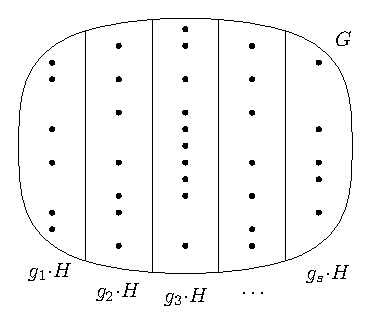
\includegraphics[width=0.3\textwidth]{AL1L24_3.eps}
			\caption{Разбиение группы $G$ на смежные классы.}
			\label{24_3}
		\end{figure}
		Таким образом, поскольку классы не пересекаются, мы получим:
		$$
			|G| = |g_1{\cdot}H| + |g_2{\cdot}H| + \dotsc + |g_s{\cdot}H| = \underbrace{|H| + |H| + \dotsc + |H|}_{s} = |H|{\cdot}s = |H|{\cdot}(G\colon H)
		$$
	\end{enumerate}
\end{proof}
\begin{rem}
	Также можно было воспользоваться леммой, которую мы рассмотрели ранее.
\end{rem}
\begin{corollary}
	Пусть $G$ - конечная группа, а $H \subseteq G$ - подгруппа, тогда: $|G| \divby|H|$.
\end{corollary}
\begin{proof}
	Очевидно: $|G| = |H|{\cdot}(G \colon H) \Rightarrow \tfrac{|G|}{|H|} = (G \colon H) \in \MN \Rightarrow |G| \divby |H|$.
\end{proof}
\begin{corollary}
	$\forall g \in G,\, |G| \divby \ord(g)$.
\end{corollary}
\begin{proof}
	Возьмем $H = \linsp{g}$, тогда $\ord(g) = |H| \Rightarrow$ применим предыдущее следствие и получим требуемое. 
\end{proof}
\begin{corollary}
	$|G| = n \Rightarrow \forall g \in G, \, g^n = e$.
\end{corollary}
\begin{proof}
	Пусть $\ord(g) = m$, тогда по следствию $2$ верно: $m \mid n, \, n = m{\cdot}d \Rightarrow g^n = (g^m)^d = e^d = e$.
\end{proof}

Пусть $m \in \MN$, рассмотрим \uwave{функцию Эйлера}: 
$$
	\varphi(m) = \{k \in 1,\dotsc, m-1 \mid (m,k) = 1\}
$$ 
Известна следующая теорема из теории чисел.
\begin{theorem}(\textbf{Эйлера})
	$\forall k \in \MZ, \, (m,k) = 1 \Rightarrow \modn{k^{\varphi(m)}}{1}{m}$.
\end{theorem}
\begin{proof}
	Рассмотрим $\MZ_m^{\times} = \{\ovl{k} \mid (k,m) = 1\}$, тогда $|\MZ_m^{\times}| = \varphi(m)$ по определению. По следствию $3$:
	$$
		\forall \ovl{k}\in \MZ_m^{\times}, \, \ovl{k}^{\varphi(m)} = \ovl{1} \Rightarrow \modn{k^{\varphi(m)}}{1}{m}
	$$
\end{proof}

Также с помощью теоремы Лагранжа можно вывести малую теорему Ферма.
\begin{corollary}(\textbf{Малая теорема Ферма})
	Пусть $p$ - простое число и $\ovl{a} \in \MZ_p$, тогда $\ovl{a}^p = \ovl{a}$.
\end{corollary}
\begin{proof}
	Рассмотрим группу $G = (\MZ_p \setminus \{0\}, \times), \, |G| = p - 1$, тогда по следствию $3$:
	$$
		\forall \ovl{a} \in \MZ_p^\times, \, \ovl{a}^{p-1} = \ovl{1} \Rightarrow \ovl{a}^p = \ovl{a}{\cdot}\ovl{a}^{p-1} = \ovl{a}{\cdot}\ovl{1} = \ovl{a}
	$$
	Но это будет выполнено и для $0 \Rightarrow$ равенство выше верно $\forall \ovl{a} \in \MZ_p$.
\end{proof}

\begin{corollary}
	Пусть $p$ - простое число, $|G| = p \Rightarrow G$ это циклическая группа, порождается любым неединичным элементом. Более точно: $G\simeq \MZ_p$, в частности, $G$ коммутативна. 
\end{corollary}
\begin{proof}
	По следствию $2$:
	$$
		\forall g \in G \setminus \{e\}, \,  |G| = p \divby |\linsp{g}| \Rightarrow |\linsp{g}| \in \{1,p\}
	$$ 
	Но $|\linsp{g}| \geq 2$, так как $e \neq g, \, e \in \linsp{g}, \, g \in \linsp{g} \Rightarrow |\linsp{g}| = p\Rightarrow \linsp{g} = G$. Коммутативность следует из коммутативности цикличных групп (циклические группы всегда коммутативны).
\end{proof}

Из теоремы Лагранжа также можно доказать для конечных групп равенство числа левых смежных классов и правых смежных классов, поскольку:
$$
	|gH| = |H| = |Hg| \Rightarrow \dfrac{|G|}{|gH|} = \dfrac{|G|}{|H|} = \dfrac{|G|}{|Hg|}
$$
Также отметим, что при этом разбиение на левые смежные классы и правые смежные классы могут не совпадать, но если $G$ - абелева, то $gH = Hg, \, \forall g \in G$.

\textbf{Пример несовпадения левых и правых смежных классов}: Рассмотрим $G = S_3, \, |G| = 6$ - это самая маленькая неабелева группа. 

Рассмотрим подгруппу: $H = A_3$ это группа всех четных подстановок (все циклы длины $3$ без транспозиций) в ней совпадут левые и правые смежные классы, поскольку $(G \colon H ) = 2$, так как $|G| = 6$, а четных подстановок в ней $3$. Поскольку $A_3$ - всегда смежный класс единицы (и левый, и правый), то:
\begin{enumerate}[label=\arabic*)]
	\item \uline{Левый смежный класс}: Половина чётные, половина нечётные;
	\item \uline{Правый смежный класс}: Тоже самое - всего два класса: половина чётные, половина нечётные;
\end{enumerate}

Рассмотрим подгруппу: $H = \linsp{(12)}  = \left\{e, 
\begin{pmatrix}
	1 & 2 & 3 \\
	2 & 1 & 3
\end{pmatrix}\right\}$, тогда её смежные классы будут устроены так:

\begin{enumerate}[label=\arabic*)]
	\item \uline{Левые}: $H = \{e,(12)\}, \, g = (13), \, (13)(12) = (123); g = (23), \, (23)(12) = (132)$;
	\item \uline{Правые}: $H = \{e,(12)\}, \, g = (13), \, (12)(13) = (132); g = (23), \,  (12)(23) = (123)$;
\end{enumerate}

\begin{exrc}
	Обратное утверждение к теореме Лагранжа не верно: пусть $G$ - конечная группа и $d$ - делитель числа $|G|$. Тогда в группе $G$ есть подгруппа $H$ у которой порядок равен $d$, то есть $|H| = d$. Привести контрпример.
\end{exrc}

\end{document}